% \newcommand{\jc}[1]{\texttt{#1}}
% \newsavebox{\titleimage}
% % \savebox{\titleimage}{\missingfigure[figwidth=12cm]}
% \savebox{\titleimage}{
%     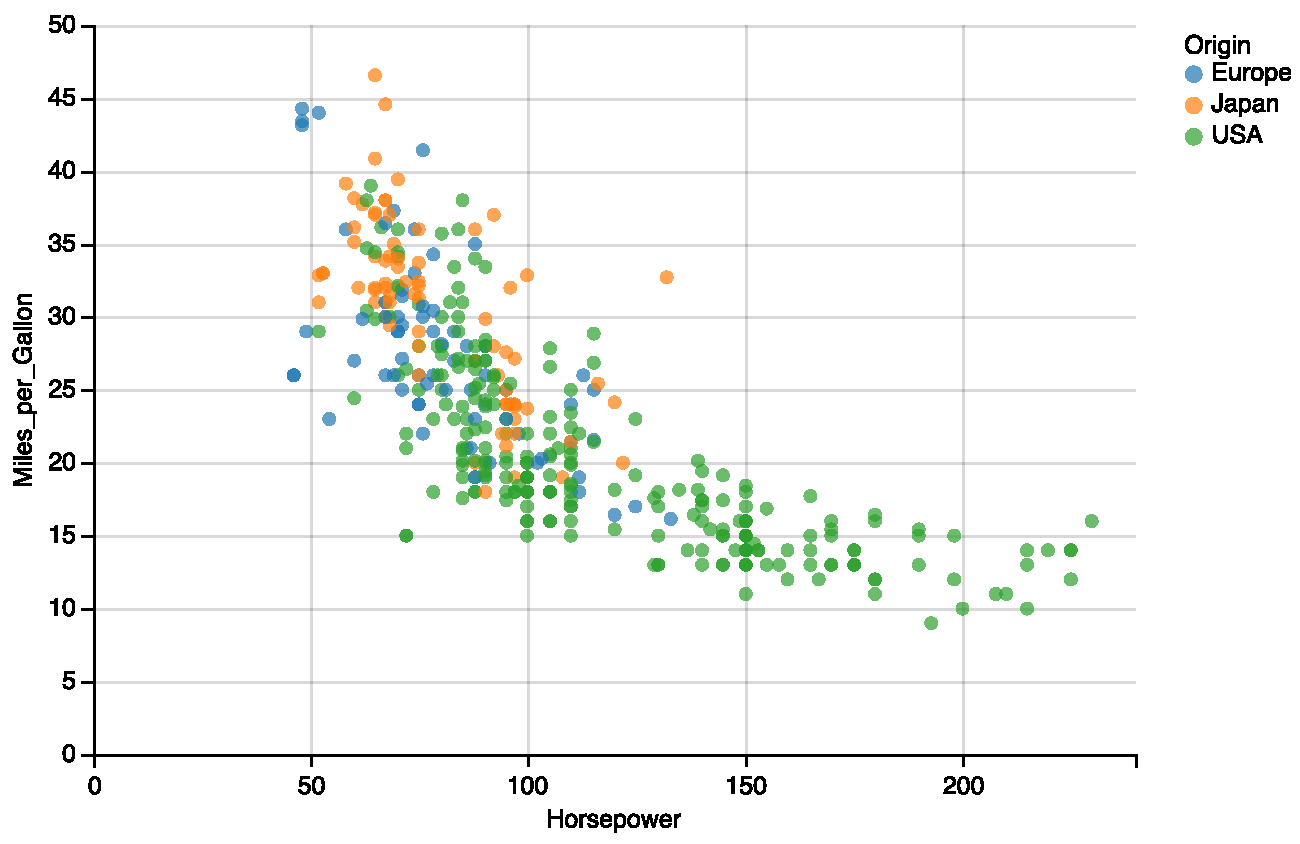
\includegraphics[width=12cm]{figures/vega.pdf}
% }
\begin{titlepage}
    \vspace*{\baselineskip}
    \vspace*{0.167\textheight} 
    Masterarbeit\\
    \vspace{\baselineskip}
    \begin{minipage}{15cm}
    {\huge Layout-Erkennung in digtalisierten Dokumenten mittels Neuronaler~Netzwerke\par}
    \end{minipage}
    
    \vspace{\baselineskip}
    von Jakob Schmolling\\
    \vfill
    Matrikelnummer:\\
    \vspace{\baselineskip}
    Datum: \today \\
    \vspace{\baselineskip}
    Fachbereich 4 Wirtschaftswissenschaften II\\
    Internationale Medieninformatik (M.A.)\\
    \vspace{\baselineskip}
    \begin{tabular}{@{\hspace{0em}}ll}
    Erstgutachter: & Prof. Dr. Klaus Jung\\
    Zweitgutachter: & Prof. Dr. Kai-Uwe Barthel\\
    \end{tabular}
\end{titlepage}
% \author{Jakob Schmolling}
% \title[]{
% \vfill
% \usebox{\titleimage}\\
% \noindent
% \huge{Layout-Erkennung in digtalisierten Dokumenten mittels Neuronaler Netzwerke}\\
% \noindent\Large{1.Korrektur}\\
% % \noindent\Large{Untertitel der Arbeit}\\
% % \noindent\Large{Untertitel der Arbeit}
% }


% \publisher[HTW Berlin]{HTW Berlin / \today}
